\chapter{Pravděpodobnost}

\section{Druhy pravděpodobnosti}

\subsection{Úvod}

Počátky teorie pravděpodobnosti jsou spojeny s hazardními hrami, jako jsou např. hod v kostky nebo ruleta. Ačkoliv podstatou hazardních her je náhoda, je zřejmé, že z dlouhodobého hlediska je možné výsledek odhadnout. Tato ``odhadnutelnost'' koneckonců umožňuje kasinu provozovat svoji činnost. S podobnou náhodností se lze setkat také v experimentální vědě, jako jsou medicína nebo fyzika.

\subsection{Klasická neboli apriorní pravděpodobnost}

Uvažujme hrací kostku. Přijetí předpokladů, že (a) při každém hodu padne číslo jedna, dva, tři, čtyři, pět nebo šest a že (b) pravděpodobnost realizace jednotlivých výsledků je shodná, vytváří model, který je možné použít k analýze hry v kostky. Modely podobného typu pak tvoří základ tzv. klasické pravděpodobnosti.

\begin{definition}[Klasická pravděpodobnost]
Uvažujme náhodný experiment, který může vyústit v $n$ vzájemně se vylučujících výsledků se shodnou pravděpodobností realizace. Jestliže $n_A$ z těchto výsledků má atribut $A$, pak je pravděpodobnost $A$ definována jako $\frac{n_A}{n}$.
\end{definition}

Výše uvedená definice má několik slabých míst. Prvním z nich je situace, kdy se $n$ popř. také $n_A$ blíží nekonečnu\footnote{Uvažujme pravděpodobnost, s jakou bude náhodně tažené přirozené číslo sudé. Je zřejmé, že tato pravděpodobnost je 0.5. Odpověď je však, spíše než na výše uvedeném vzorci, založena na intuici.}. Další komplikací jsou případy, kdy jednotlivé výsledky nemají shodnou pravděpodobnost realizace. Vzorec $\frac{n_A}{n}$ také není vhodný, jestliže potřebujeme určit tzv. podmíněnou pravděpodobnost. Z těchto důvodů byla vyvinuta teorie posteriorní pravděpodobnosti.

\subsection{Posteriorní pravděpodobnost}

V případě apriorní pravděpodobnosti jsme si vytvořili mentální model hrací kostky, které jsme přisoudili určité vlastnosti. Při každém hodu mohlo nastat šest vzájemně se vylučujících výsledků, kterým jsme přiřadili shodnou pravděpodobnost, tj. $\frac{1}{6}$.

K problému je však možné přistupovat také z druhé strany. Definujme pravděpodobnost hodu konkrétního čísla jako $p_i$, kde $i = 1, 2,..., 6$. Abychom tyto pravděpodobnosti určili pro jednu konkrétní hrací kostku, proveďme velké množství hodů a jejich výsledky zaznamenejme. Frekvenci jednotlivých čísel pak použijeme jako odhad pravděpodobnosti $p_i$. Vzhledem k tomu, že jsme pravděpodobnost neurčili a priori (tj. pouze na základě logického zhodnocení modelu) ale ex-post (na základě zkušenosti s konkrétní hrací kostkou), hovoříme o tzv. posteriorní pravděpodobnosti. Je zřejmé, že pokud bude daná hrací kostka správně vyvážená a počet kontrolních hodů dostatečně velký, budou posteriorní pravděpodobnosti přibližně odpovídat apriorním pravděpodobnostem.

\section{Axiomy pravděpodobnosti}

\subsection{Pravděpodobnostní modely}

Apriorní a posteriorní pravděpodobnost jsou vztaženy k experimentu, který je možné opakovat v homogenním prostředí. Jako příklad jsme uváděli hod hrací kostkou. V řadě případů však pravděpodobnost není možné podrobit opakovaným experimentům. Příkladem budiž pravděpodobnost, s jakou ve vesmíru existuje inteligentní život mimo Zemi. Vzhledem k tomu, že tyto pravděpodobnosti nelze přesně kvatifikovat, hovoříme o nich jako o subjektivní pravděpodobnosti. Ačkoliv je subjektivní pravděpodobnost legitimní součástí obecné teorie pravděpodobnosti, zaměřuje se tato kniha přávě na apriorní a posteriorní pravděpodobnost.

Experiment, jehož výstupem jsou náhodné výsledky, tvoří základ pro tzv. pravděpodobnostní model. V jeho rámci definujeme všechny možné výsledky experimentu, tzv. elementární jevy. Jestliže se vrátíme k našemu příkladu hrací kostky, jsou elementární jevy definované hody 1, 2, 3, 4, 5 a 6\footnote{Situace, kdy se hrací kostka zastaví na hraně nebo se v průběhu hodu ztratí, ignorujeme - v našem pravděpodobnostním modelu nemohou nastat, a proto jim přiřazujeme pravděpodobnost nula.}. Elementární jevy pak tvoří tzv. výběrový prostor. Množinovými operacemi nad elementárními jevy definujeme tzv. náhodné jevy. Příkladem náhodného jevu v kontextu hrací kostky je např. situace, kdy padne
\begin{itemize}
\item sudé číslo,
\item číslo větší než dvě,
\item číslo dvě\footnote{V tomto případě je náhodný jev tvořený jedním elementárním jevem. V přechozích příkladech byl náhodný jev tvořen množinou elementárních jevů.}.
\end{itemize}
Všechny myslitelné náhodné jevy pak tvoří tzv. jevové pole.

\subsection{Teorie množin}

Uvažujme soubor objektů, který je dostatečně velký na to, aby obsahoval každý jednotlivý objekt relevantní pro daný problém. Každý jednotlivý objekt označme jako prvek $\omega$ a jejich úplný soubor jako pole $\Omega$.

Skupina prvků definuje množinu. Skutečnost, že prvek $\omega$ patří do množiny $A$, označujeme jako $\omega \in A$.

\begin{definition}[Podmnožina]
Uvažujme množiny $A$ a $B$. Jestliže každý prvek mnnožiny $A$ je současně prvkem množiny $B$, pak o množině $A$ hovoříme jako o podmnožině množiny $B$. Tuto skutečnost značíme jako $A \subset B$.
\end{definition}

\begin{definition}[Ekvivalentní množiny]
Uvažujme množiny $A$ a $B$. Jestliže současně platí $A \subset B$ a $B \subset B$, pak je každý prvek množiny $A$ současně prvkem množiny $B$ a naopak. Množiny $A$ a $B$ jsou tzv. ekvivalentní. Tuto skutečnost značíme jako $A = B$.
\end{definition}

\begin{definition}[Prázdná množina]
Jestliže množina neobsahuje žádný prvek, nazýváme ji prázdnou množinou a označujeme jako $\emptyset$.
\end{definition}

\begin{definition}[Doplněk množiny]
Doplněk množiny $A$ vzhledem k poli $\Omega$, označujeme jako $A^{c}$ nebo také jako $\Omega - A$. Doplněk představuje množinu všech prvků, které jsou obsaženy v poli $\Omega$ a zároveň nejsou obsaženy v množině $A$.
\end{definition}

\begin{definition}[Sjednocení množin]
Nechť jsou $A$ a $B$ libovolné podmnožiny pole $\Omega$. Množinu tvořenou všemi prvky obsaženými v množině $A$ nebo v množině $B$, nazýváme sjednocením množin $A$ a $B$ a značíme jako $C = A \cup B$.
\end{definition}

\begin{definition}[Průnik množin]
Nechť jsou $A$ a $B$ libovolné podmnožiny pole $\Omega$. Množinu tvořenou všemi prvky současně obsaženými v množině $A$ a množině $B$, nazýváme průnikem množin $A$ a $B$ a značíme jako $C = A \cap B$.
\end{definition}

\begin{definition}[Rozdíl množin]
Nechť jsou $A$ a $B$ libovolné podmnožiny pole $\Omega$. Množinu tvořenou všemi prvky, které jsou obsaženy v množině $A$ a zároveň nejsou obsaženy v množině $B$, nazýváme rozdílem množin $A$ a $B$ a značíme jako $C = A - B$.
\end{definition}

\begin{theorem}[Pravidlo komutace]
\begin{equation*}
A \cup B = B \cup A
\end{equation*}
\begin{equation*}
A \cap B = B \cap A
\end{equation*}
\end{theorem}

\begin{theorem}[Pravidlo asociace]
\begin{equation*}
A \cup (B \cup C) = (A \cup B) \cup C
\end{equation*}
\begin{equation*}
A \cap (B \cap C) = (A \cap B) \cap C
\end{equation*}
\end{theorem}

\begin{theorem}[Pravidlo distribuce]
\begin{equation*}
A \cap (B \cup C) = (A \cap B) \cup (A \cap B)
\end{equation*}
\begin{equation*}
A \cup (B \cap C) = (A \cup B) \cap (A \cup B)
\end{equation*}
\end{theorem}

\begin{theorem}
Doplněk k doplňku množiny $A$ je roven množině $A$.
\begin{equation*}
(A^c)^c = A
\end{equation*}
\end{theorem}

\begin{theorem}
\begin{equation*}
A \cap \Omega = A
\end{equation*}
\begin{equation*}
A \cup \Omega = \Omega
\end{equation*}
\begin{equation*}
A \cap \emptyset = \emptyset
\end{equation*}
\begin{equation*}
A \cup \emptyset = A
\end{equation*}
\end{theorem}

\begin{theorem}
\begin{equation*}
A \cap  A^c = \emptyset 
\end{equation*}
\begin{equation*}
A \cup A^c = \Omega
\end{equation*}
\begin{equation*}
A \cap A = A
\end{equation*}
\begin{equation*}
A \cup A = A
\end{equation*}
\end{theorem}

\begin{theorem}[De Morganovo pravidlo]
\begin{equation*}
(A \cup B)^c = A^c \cap B^c
\end{equation*}
\begin{equation*}
(A \cap B)^c = A^c \cup B^c
\end{equation*}
\end{theorem}

\begin{theorem}
\begin{equation*}
A - B = A \cap B^c
\end{equation*}
\end{theorem}

\begin{proof}
Dokažme, že $(A \cup B)^c = A^c \cap B^c$. Dle definice jsou dvě množiny shodné, jestliže je každá z nich obsažena ve té druhé, tj. $A \subset B$ a zároveň $B \subset A$. Jestliže $\omega \in (A \cup B)^c$, pak $\omega \in A^c \cap B^c$. Platí tedy, že $(A \cup B)^c \subset A^c \cap B^c$. Dále $\omega \in (A \cup B)^c$ implikuje $\omega \notin A \cup B$, což implikuje $\omega \notin A$ a $\omega \notin B$, což implikuje $\omega \in A^c \cap B^c$. Dalším krokem je prokázat, že $A^c \cap B^c \subset (A \cup B)^c$. Nechť $\omega \in A^c \cap B^c$, což znamená, že $\omega$ patří do $A^c$ i do $B^c$. Pak $\omega \notin A \cup B$, protože $\omega$ by muselo patřit do $A$ nebo do $B$. To popírá skutečnost, že $\omega$ patří současně do $A^c$ a $B^c$. Nicméně $\omega \notin A \cup B$ znamená $\omega \in (A \cup B)^c$, čímž jsme prokázali požadované.
\end{proof}

\begin{figure}[htp]
\centering
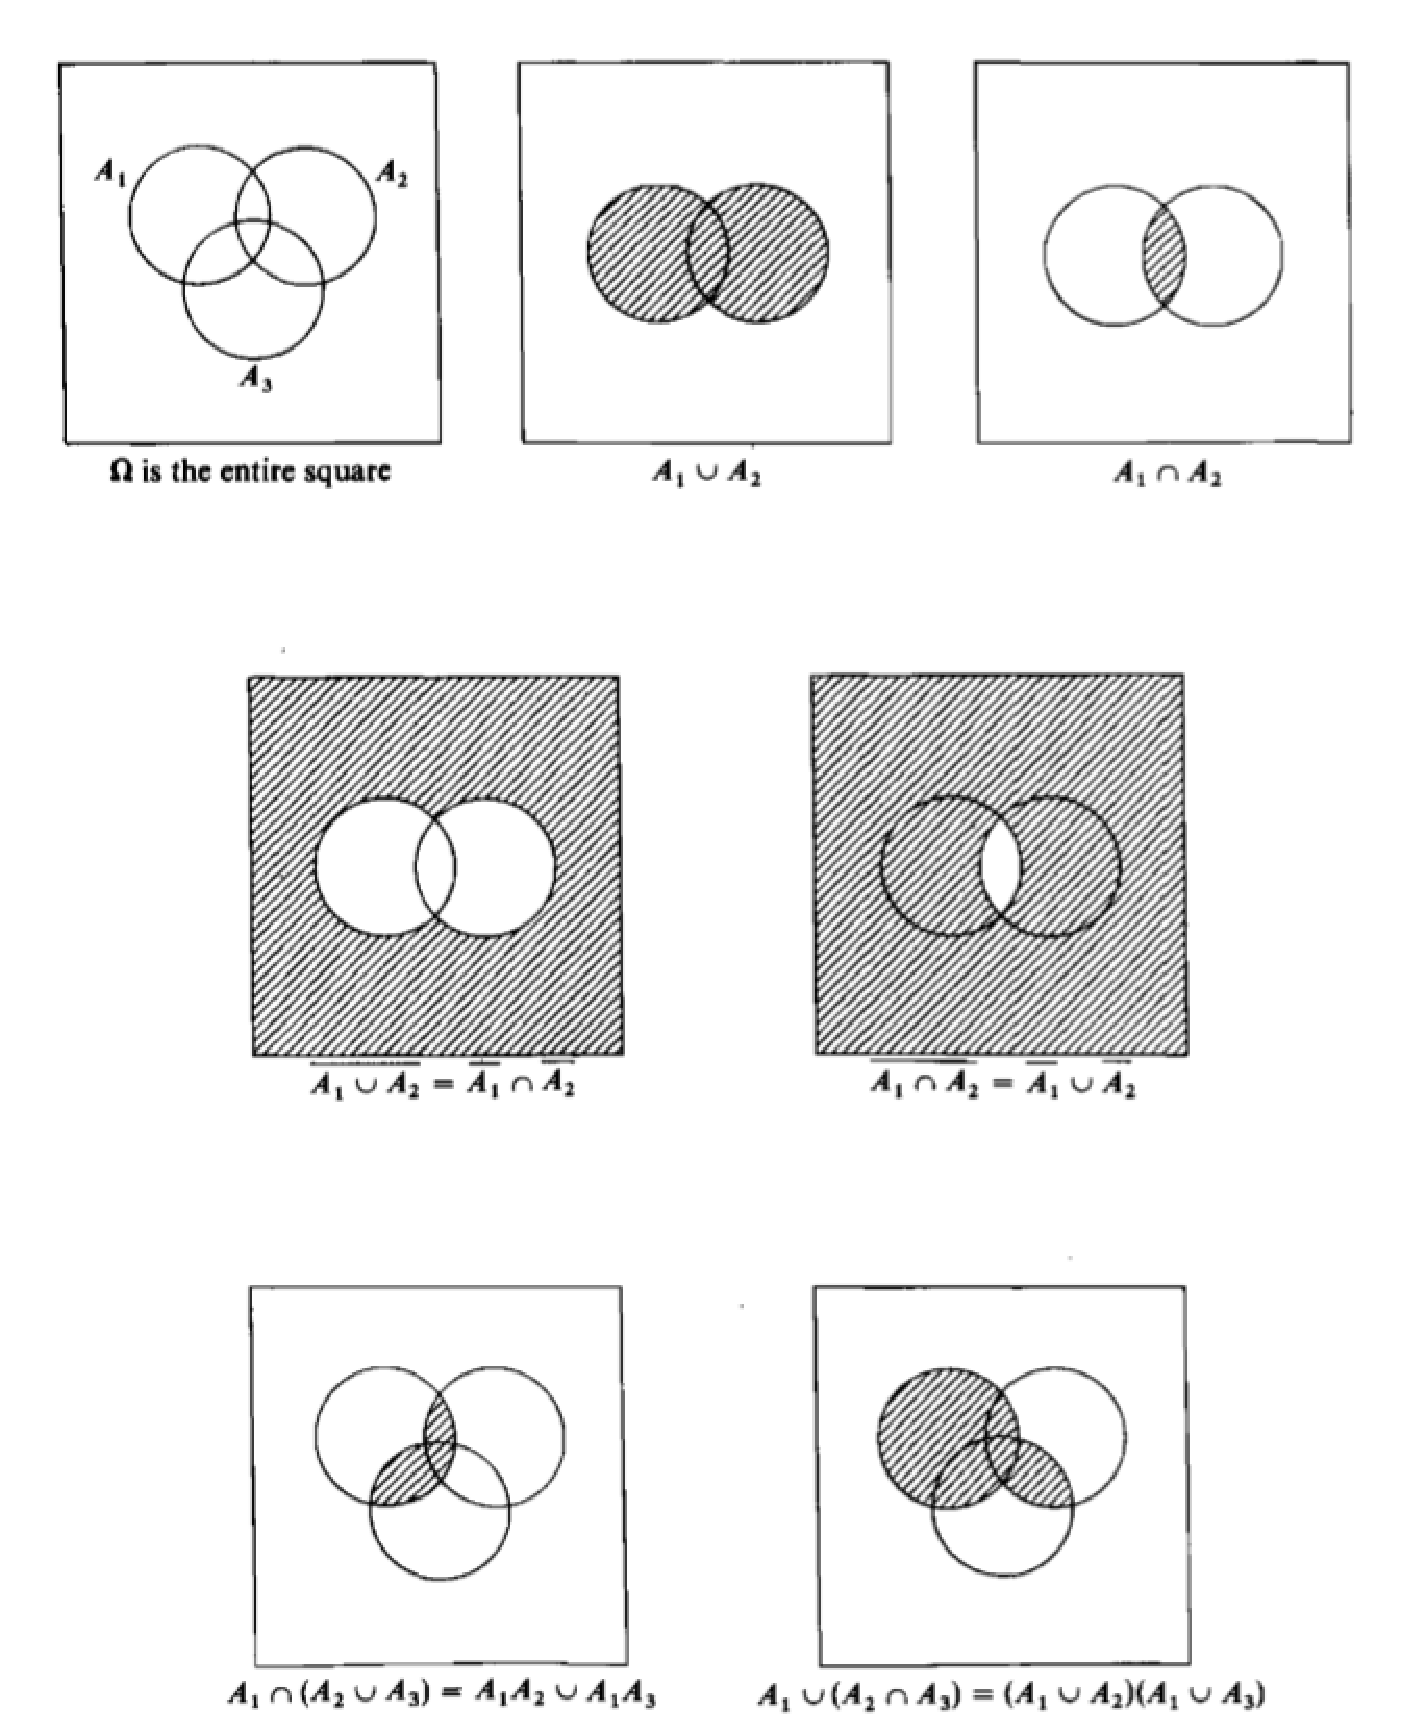
\includegraphics[scale = 0.5]{pictures/set_operations.eps}
\caption{Množinové operace nad náhodnými jevy}
\label{set_operations}
\end{figure} 

Je zvykem rozlišovat jednotlivé množiny v v poli $\Omega$ přiřazením indexů. Označme množinu takovýchto indexů jako $\Lambda$. Jestliže bychom uvažovali pouze dvě podmnožiny pole $\Omega$, pak bude $\Lambda$ obsahovat pouze dva indexy, řekněme $\Lambda = {1, 2}$.

\begin{definition} [Sjednocení a průnik množin]
Nechť $\Lambda$  je množinou indexů a $\{A_{\lambda}: \lambda \in \Lambda\} = \{A_{\lambda}\}$ je souborem podmnožin pole $\Omega$ indexovaných dle $\Lambda$. Množinu, která obsahuje všechny prvky náležící do alespoň jednoho $A_{\lambda}$, nazýváme sjednocením množin $\{A_{\lambda}\}$ a značíme jako $\bigcup_{\lambda \in \Lambda} A_{\lambda}$. Množinu, která obsahuje všechny prvky současně náležících do všech $A_{\lambda}$, nazýváme průnikem množin $\{A_{\lambda}\}$ a značíme jako $\bigcap_{\lambda \in \Lambda} A_{\lambda}$. Jestliže je $\Lambda$ prázdnou množinou, pak definujeme sjednocení jako $\bigcup_{\lambda \in \Lambda} A_{\lambda} = \emptyset$ a průnik jako $\bigcap_{\lambda \in \Lambda} A_{\lambda} = \Omega$.
\end{definition}

\begin{theorem}[De Morganův theorém]
Nechť $\Lambda$ představuje množinu indexů a $\{A_{\lambda}\}$ je souborem všech podmnožin pole $\Omega$ indexovaných dle $\Lambda$. Pak
\begin{equation*}
\Big(\bigcup_{\lambda \in \Lambda} A_{\lambda}\Big)^c = \bigcap_{\lambda \in \Lambda} A^c_{\lambda}
\end{equation*}
\begin{equation*}
\Big(\bigcap_{\lambda \in \Lambda} A_{\lambda}\Big)^c = \bigcup_{\lambda \in \Lambda} A^c_{\lambda}
\end{equation*}
\end{theorem}

\begin{definition}[Disjuktní množiny]
Podmnožiny $A$ a $B$ pole $\Omega$ jsou disjuktní, jestliže $A \cap B = \emptyset$. Podmnožiny $A_1$, $A_2, ...$ jsou vzájemně disjuktní, jestliže $A_i \cap A_j = \emptyset$ pro všechna $i \not= j$.  
\end{definition}

\begin{theorem}
Jestliže jsou $A$ a $B$ podmnožiny pole $\Omega$, pak
\begin{enumerate}
\item $A = (A \cap B) \cup (A \cap B^c)$
\item $(A \cap B) \cap (A \cap B^c) = \emptyset$
\end{enumerate}
\end{theorem}

\begin{proof}
~
\begin{enumerate}
\item $A = A \cap \Omega = A \cap (B \cup B^c) = (A \cap B) \cup (A \cap B^c)$
\item $(A \cap B) \cap (A \cap B^c) = (A \cap A) \cap (B \cap B^c) = A \cap \emptyset = \emptyset$
\end{enumerate}
\end{proof}
\begin{theorem}
Jestliže $A \subset B$, pak $A \cap B = A$ a $A \cup B = B$.
\end{theorem}

\subsection{Definice výběrového prostoru a náhodného jevu}

\begin{definition}[Výběrový prostor]
Výběrový prostor, označovaný jako $\Omega$, představuje soubor všech možných výstupů náhodného experimentu.
\end{definition}

\begin{definition}[Náhodný jev a jevové pole]
Náhodný jev je podmnožinou výběrového prostoru. Množina všech náhodných jevů souvisejících s daným experimentem pak představuje jevové pole tohoto experimentu.
\end{definition}

Výše uvedená definice přesně nevymezuje pojem ``náhodný jev''. Náhodný jev je vždy podmnožinou výběrového prostoru, avšak pro dostatečně velký výběrový prostor ne všechny jeho podmnožiny musí představovat náhodný jev. Proto soubor všech podmnožin výběrového prostoru nemusí nutně odpovídat jevovému poli. Nicméně množina všech náhodných jevů může být vždy zvolena dostatečně velká na to, aby obsahovala všechny náhodné jevy, jejichž pravděpodobností bychom se mohli chtít zabývat. Jestliže se výběrový prostor skládá z konečného počtu prvků, pak odpovídající jevové pole bude množinou všech podmnožin výběrového prostoru.

Naším primárním zájmem je pravděpodobnost, s jakou určitý náhodný jev nastane popř. nenastane. Náhodný jev $A$ nastane, jestliže výsledek experimentu (tj. prvek odpovídajícího výběrového prostoru) náleží $A$. Protože prvek $\omega$ výběrového prostoru $\Omega$ je z definice jeho podmnožinou, je zároveň kandidátem pro náhodný jev. Proto můžeme na $\omega$ nahlížet jako na prvek i jako na podmnožinu $\Omega$. Abychom tyto dva možné pohledy odlišili, používáme značení $\omega$, jestliže mluvíme o prvku, a značení $\{\omega\}$, jestliže mluvíme o podmnožině. Také $\emptyset$ a $\Omega$  jsou podmnožinami $\Omega$ a jsou tak náhodnými jevy. $\Omega$ někdy nazýváme jistým jevem.

Pro značení náhodných jevů se zpravidla používají velká písmena latinské abecedy (s výjimkou výše zmíněných $\emptyset$ a $\Omega$), tj. např. $A$. Jevové pole je pak nejčastěji označeno skriptovým písmenem latinské abecedy jako např. $\mathscr{A}$.

Jevové pole $\mathscr{A}$ by mělo splňovat
\begin{enumerate}
\item $\Omega \in \mathscr{A}$,
\item je-li $A \in \mathscr{A}$, pak $A^c \in \mathscr{A}$ a
\item jestliže $A_1 \in \mathscr{A}$ a $A_2 \in \mathscr{A}$, pak $A_1 \cup A_2 \in \mathscr{A}$.
\end{enumerate}
Jakýkoliv souhrn náhodných jevů, které splňují výše uvedené tři podmnínky, nazýváme algebrou náhodných jevů, zkráceně též algebrou. Je zřejmé, že soubor všech podmnožin výběrového prostoru $\Omega$ splňuje tyto podmínky. Tyto požadované vlastnosti pak implikují následující vlastnosti jevového pole $\mathscr{A}$.

\begin{theorem}
$\emptyset \in \mathscr{A}$
\end{theorem}
\begin{proof}
Uvažujme vlastnost (1) $\Omega \in \mathscr{A}$ a související vlastnost (2) $\Omega^c \in \mathscr{A}$. Nicméně $\Omega^c = \emptyset$, a proto $\emptyset \in \mathscr{A}$.
\end{proof}
\begin{theorem}
Jestliže $A_1 \in \mathscr{A}$ a $A_2 \in \mathscr{A}$, pak $A_1 \cap A_2 \in \mathscr{A}$.
\end{theorem}
\begin{proof}
Platí $A_1^c \in \mathscr{A}$ a $A_2^c \in \mathscr{A}$, což implikuje $A_1^c \cup A_2^c \in \mathscr{A}$ a $(A_1^c \cup A_2^c)^c \in \mathscr{A}$. Zároveň, dle De Morganova pravidla, platí $(A_1^c \cup A_2^c)^c = A_1^c \cap A_2^c = A_1 \cap A_2$.
\end{proof}
\begin{theorem}
Jestliže $A_1, A_2, ..., A_n \in \mathscr{A}$, pak $\cup^{n}_{i=1}A_i \in \mathscr{A}$ a $\cap^{n}_{i=1}A_i \in \mathscr{A}$.
\end{theorem}
V následujícím textu budeme vždy předpokládat, že souhrn všech jevů $\mathscr{A}$ je algebra. V praxi lze algebru $\mathscr{A}$ vytvořit tak, že soubor jevů, o které se zajímáme, rozšíříme o
\begin{enumerate}
\item jistý jev,
\item všechny komplementární jevy a
\item a všechna konečná sjednocení a průniky těchto jevů.
\end{enumerate}
Až dosud jsme nevysvětlili, proč $\mathscr{A}$ není vždy souborem všech podmnožin výběrového prostoru $\Omega$. Vysvětlení poskytneme v následující kapitole.

\subsection{Definice pravděpodobnosti}

\begin{definition}[Funkce]
Funkce $f(\cdot)$ s definičním oborem $A$ a oborem hodnot $B$ je souborem uspořádaných párů $(a, b)$, které splňují
\begin{enumerate}
\item $a \in A$ a $b \in B$,
\item pro každé $a \in A$ existuje uspořádaný pár $(a, b)$\footnote{Obrácené tvrzení však neplatí. Nelze tedy říci, že pro každé $b \in B$ existuje uspořádaný pár $(a, b)$.} a
\item žádné dva uspořádané páry nemají shodný první element\footnote{To znamená, že neexistují dvě uspořádané dvojice $(a, b_1)$ a $(a, b_2)$, kde $b_1 \not= b_2$.}.
\end{enumerate}
\end{definition}

Jestliže $(a, b) \in f(\cdot)$, píšeme $b = f(a)$ a $f(a)$ nazýváme hodnotou funkce $f(\cdot)$ v bodě $a$. Pro libovolné $a \in A$ platí $f(a) \in B$. Označením $f(\cdot)$ rozumíme uspořádaný pár $(a, b = f(a))$. $f(a)$ někdy také nazýváme obrazem bodu $a$ pro $f(\cdot)$.

\begin{definition}[Indikační funkce]
Nechť $\Omega$ představuje prostor s body $\omega$ a $A$ představuje libovolnou podmnožinu $\Omega$. Indikační funkce $A$, označována jako $I_A(\cdot)$, je funkcí s definičním oborem $\Omega$ a oborem hodnot $\{0, 1\}$ a je definována jako
\begin{equation*}
I_A(\omega) = 
\begin{cases}
1~~~\textit{pro}~\omega \in A \\
0~~~\textit{pro}~\omega \notin A
\end{cases}
\end{equation*}
\end{definition}

Nechť $\Omega$ představuje libovolný výběrový prostor a $\mathscr{A}$ libovolný soubor podmnožin $\Omega$. Pak
\begin{enumerate}
\item $I_A(\omega) = 1 - I_{A^c}(\omega)$ pro všechna $A \in \mathscr{A}$,
\item $I_{A_1 \cap A_2 \cap \cdots \cap A_n}(\omega) = I_{A_1}(\omega) \cdot I_{A_2}(\omega) \cdots I_{A_n}(\omega)$ pro $A_1, A_2, ..., A_n \in \mathscr{A}$,
\item $I_{A_1 \cup A_2 \cup \cdots \cup A_n}(\omega) = \max[I_{A_1}(\omega), I_{A_2}(\omega), ..., I_{A_n}(\omega)]$ pro $A_1, A_2, ..., A_n \in \mathscr{A}$ a
\item $I^2_A(\omega) = I_A(\omega)$ pro všechna $A \in \mathscr{A}$.
\end{enumerate}

Indikační funkci lze použít také pro ``indikaci'' podmnožin reálné osy
\begin{equation*}
I_{[0,1]}(x) =
\begin{cases}
1~~~\textit{pro}~ 0 \le x < 1\\
0~~~\textit{v ostatních případech}
\end{cases}
\end{equation*}
popř. množiny přirozených čísel
\begin{equation*}
I_{I^+}(x) =
\begin{cases}
1~~~\textit{jestliže $x$ je přirozené číslo}\\
0~~~\textit{v ostatních případech}
\end{cases}
\end{equation*}

Pro následujicí text předpokládáme, že $\Omega$ označuje výběrový prostor a $\mathscr{A}$ označuje souhrn jevů, které představují algebru pro určitý náhodný experiment.

\begin{definition}[Pravděpodobnostní funkce]
Pravděpodobnostní funkce $P[\cdot]$ je funkcí s definičním oborem $\mathscr{A}$ a oborem hodnot $[0, 1]$, která splňuje axiomy
\begin{enumerate}
\item $P[A] \ge 0$ pro každé $A \in \mathscr{A}$,
\item $P[\Omega] = 1$ a
\item jsou-li $A_1, A_2, ...$ vzájemně neslučitelné jevy\footnote{Jevy $A_i$ a $A_j$ jsou vzájmně neslučitelné, jestliže nemohou nastat současně, tj. $A_i \cap A_j = \emptyset$ pro $i \not= j$.} v $\mathscr{A}$ a jestliže $A_1 \cup A_2 \cup \cdots = \cup_{i=1}^{\infty}A_i \in \mathscr{A}$, pak $P[\cup_{i=1}^{\infty}A_i] = \sum_{i=1}^{\infty}P[A_i]$.
\end{enumerate}
\end{definition}

V naší definici náhodného jevu a jevového pole $\mathscr{A}$ jsme zmínili, že $\mathscr{A}$ nemůže být vždy chápáno jako souhrn všech podmnožin $\Omega$. Důvodem je skutečnost, že pro ``dostatečně velké'' $\Omega$ je soubor všech podmnožin v $\Omega$ příliš velký a je tak nemožné definovat pravděpodobnostní funkci, která by byla konzistentní s výše uvedenými axiomy. Tyto axiomy implikují následující věty.

\begin{theorem}
$P[\emptyset] = 0$
\end{theorem}
\begin{proof}
Uvažujme $A_1 = \emptyset$, $A_2 = \emptyset, ...$. Pak dle axiomu (3) platí
\begin{equation*}
P[\emptyset] = P[\cup_{i=1}^{\infty}A_i] = \sum_{i=1}^{\infty}P[A_i] = \sum_{i = 1}^{\infty}P[\emptyset]
\end{equation*}
což platí, pouze je-li $P[\emptyset] = 0$.
\end{proof}
\begin{theorem}
Jestliže jsou $A_1, ..., A_n$ vzájemně neslučitelné jevy v $\mathscr{A}$, pak
\begin{equation*}
P[A_1 \cup \cdots \cup A_n] = \sum_{i=1}^n P[A_i]
\end{equation*}
\end{theorem}
\begin{proof}
Nechť $A_{n+1} = \emptyset, A_{n+2} = \emptyset, ...$. Pak $\cup_{i = 1}^nA_i = \cup_{i = 1}^{\infty}A_i \in \mathscr{A}$ a
\begin{equation*}
P[\cup_{i=1}^n A_i] = P[\cup_{i=1}^{\infty}A_i] = \sum_{i=1}^{\infty}P[A_i] = \sum_{i=1}^nP[A_i]
\end{equation*}
\end{proof}
\begin{theorem}
Jestliže je $A$ jevem z jevového pole $\mathscr{A}$, pak
\begin{equation*}
P[A^c] = 1 - P[A]
\end{equation*}
\end{theorem}
\begin{proof}
$A \cup A^c = \Omega$ a $A \cap A^c = \emptyset$. Proto
\begin{equation*}
P[\Omega] = P[A \cup A^c] = P[A] + P[A^c]
\end{equation*}
Zároveň však platí $P[\Omega] = 1$, čímž jsme dokázali požadované.
\end{proof}
\begin{theorem}
Jestliže $A \in \mathscr{A}$ a $B \in \mathscr{A}$, pak
\begin{equation*}
P[A] = P[A \cap B] + P[A \cap B^c]
\end{equation*}
a
\begin{equation*}
P[A-B] = P[A \cap B^c] = P[A] - P[A \cap B]
\end{equation*}
\end{theorem}
\begin{proof}
$A = A \cap B \cup A \cap B^c$ a $(A \cap B) \cup (A \cap B^c) = \emptyset$. Proto $P[A] = P[A \cap B] + P[A \cap B^c]$.
\end{proof}
\begin{theorem}
Pro každé dva jevy $A \in \mathscr{A}$ a $B \in \mathscr{A}$ platí $P[A \cap B] = P[A] + P[B] - P[A \cap B]$. Tuto větu lze zobecnit do tvaru
\begin{gather*}
P[A_1 \cup A_2 \cup \cdots \cup A_n] = \sum_{j=1}^n P[A_j] - \sum \sum_{i<j}P[A_i \cap A_j] + \\ +\sum \sum \sum_{i<j<k}P[A_i \cap A_j \cap A_k] - \cdots + (-1)^{n+1}P[A_1 \cap A_2 \cap \cdots \cap A_n]
\end{gather*}
\end{theorem}
\begin{proof}
Platí $A \cup B = A \cup (A^c \cap B)$ a $A \cap (A^c \cap B) = \emptyset$. Proto
\begin{equation*}
P[A \cup B] = P[A] + P[A^c \cap B] = P[A] + P[B] - P[A \cap B]
\end{equation*}
Zobecněnou verzi věty lze dokázat pomocí indukce.
\end{proof}
\begin{theorem}
Jestliže $A \in \mathscr{A}$ a $B \in \mathscr{A}$ a $A \subset B$, pak $P[A] \le P[B]$.
\end{theorem}
\begin{proof}
Platí $B = (B \cap A) \cup (B \cap A^c)$ a $A = B \cap A$. Proto $B = A \cup (B \cap A^c)$ a $A \cap (B \cap A^c) = \emptyset$, což implikuje $P[B]=P[A]+P[B \cap A^c]$. Důkaz završíme zjištěním, že $P[B \cap A^c] \ge 0$.
\end{proof}
\begin{theorem}[Booleova nerovnost]
Jestliže $A_1, A_2, ..., A_n \in \mathscr{A}$, pak
\begin{equation*}
P[A_1 \cup A_2 \cup \cdots \cup A_n] \le P[A_1] + P[A_2] + \cdots + P[A_n]
\end{equation*}
\end{theorem}
\begin{proof}
Platí $P[A_1 \cup A_2] = P[A_1] + P[A_2] - P[A_1 \cap A_2] \le P[A_1] + P[A_2]$. Důkaz lze dokončit pomocí indukce.
\end{proof}
\begin{definition}[Pravděpodobnostní prostor]
Pravděpodobnostní prostor je definován tripletem $(\Omega, \mathscr{A}, P[\cdot])$, kde $\Omega$ představuje výběrový prostor, $\mathscr{A}$ jevové pole a $P[\cdot]$ pravděpodobnostní funkci s definičním oborem $\mathscr{A}$.
\end{definition}

\subsection{Konečný výběrový prostor}

Nechť $\omega_1, \omega_2, ..., \omega_n$ představují elemetární jevy konečného výběrového prostoru $\Omega$. Uvažujme funkci $P[\cdot]$ s definičním oborem tvořeným souborem všech podmnožin prostoru $\Omega$, která splňuje následující podmínky
\begin{enumerate}
\item $P[\{\omega_1\}] = P[\{\omega_2\}] = \cdots = P[\{\omega_N\}]$
\item Je-li $A$ podmnožinou $\Omega$ obsahující $N(A)$ elementárních jevů, pak $P[A] = N(A)/N$.
\end{enumerate}
Lze relativně snadno dokázat, že funkce $P[\cdot]$ splňuje všechny tři axiomy kladené na pravděpodobnostní funkce, a proto je pravděpodobnostní funkcí.

\begin{definition}[Pravděpodobnostní funkce se shodnou pravděpodobností]
Pravděpodobnostní funkce $P[\cdot]$, která splňuje výše uvedené dvě podmínky, je tzv. pravděpodobnostní funkcí se shodnou pravděpodobností.
\end{definition}

Uvažujme experiment, jehož výsledkem je vzorek o velikosti $n$. Myšlenku lze ilustrovat na příkladu nádoby obsahující $M$ míčků, ze které je náhodně taženo $n$ míčků. Existují dva základní způsoby výběru vzorku a to s vracením (po té, co je míček vybrán, je vrácen zpět do nádoby) a bez vracení (po té, co je míček vybrán, je odložen stranou). Jestliže bude záležet na pořadí, v jakém jsou míčky taženy, pak v případě náhodného výběru s vracením existuje $M^n = \underbrace{M \cdots M}_n$ a v případě náhodného výběru bez vracení $(M)_n = M(M - 1) \cdots (M - n + 1)$ $n$-tic. Jestliže na pořadí, v jakém jsou míčky taženy, nezáleží, existuje v případě výběru s vracením $\frac{M^n}{n!}$ a v případě výběru bez vracení $\binom{M}{n} = \frac{(M)_n}{n!}$ $n$-tic. $n$-tice, u kterých záleží na pořadí, nazýváme uspořádané, a $n$-tice, u kterých na pořadí nezáleží, nazýváme neuspořádané.

\begin{example}
Uvažujme množinu $S$ o $M$ prvcích. Celkový počet podmnožin množiny $S$ je roven $\sum_{n = 0}^M \binom{M}{n}$. Pro  $a = b = 1$ je z binomické věty $(a + b)^M = \sum_{n=0}^M \binom{M}{n}a^nb^{M-n}$ zřejmé, že $2^M = \sum_{n=0}^M \binom{M}{n}$. Množina o $M$ prvcích tak má $2^M$ podmnožin.
\end{example}

Uvažujme situaci, kdy nádoba obsahuje $M$ míčků, z nichž právě $K$ je bílých. Pravděpodobnost, že při výběru $n$ míčků s vracením jich bude právě $k$ bílých, je rovna
\begin{equation*}
\frac{\binom{n}{k}K^k(M-K)^{n-k}}{M^n}
\end{equation*}
Pří výběru bez vracení je tato pravděpodobnosti rovna
\begin{equation*}
\frac{\binom{n}{k}(K)_k(M-K)_{n-k}}{(M)_n} = \frac{\binom{K}{k}\binom{M-K}{n-k}}{\binom{M}{n}}
\end{equation*}
Pro úplnost dodejme, že v kontextu výše uvedených dvou rovnic je pořadí, v jakém jsou míčky taženy, irelevantní.

Až dosud jsme uvažovali, že pravděpodobnost realizace jednotlivých výsledků náhodného experimentu jsou shodné. V řadě případů však tento předpoklad nemusí být splněn. Nechť $\Omega = \{\omega_1, ..., \omega_2\}$ a předpokládejme $p_j = P[\{ \omega_j\}]$ pro $j = 1, ..., N$. Proto
\begin{equation*}
1 = P[\Omega] = P \big[\cup_{j=1}^N \{\omega_j \} \big] = \sum_{j = 1}^N P[\{ \omega_j \}] = \sum_{j = 1}^N p_j
\end{equation*}
Pro libovolný jev $A$ pak definujeme $P[A] = \sum p_j$, kde sumace jde přes ta $\omega_j$, která náleží $A$. Lze dokázat, že takto definovaná $P[\cdot]$ splňuje všechny tři axiomy pravděpodobnostní funce, a proto je pravděpodobnostní funkcí.

\subsection{Podmíněná pravděpodobnost a nezávislost}

\begin{definition}[Podmíněná pravděpodobnost]
Nechť $A$ a $B$ jsou dva jevy z $\mathscr{A}$ pro pravděpodobnostní prostor $(\Omega, \mathscr{A}, P[\cdot])$. Podmíněná pravděpodobnost jevu $A$ za předpokladu realizace jevu $B$ je definována jako
\begin{equation*}
P[A|B] = \frac{P[A \cap B]}{P[B]}~~~\textit{pro}~P[B] > 0
\end{equation*}
V případě $P[B] = 0$ není tato pravděpodobnost definována. 
\end{definition}
Z výše uvedeného je zřejmé, že $P[A \cap B] = P[A|B]P[B] = P[B|A]P[A]$ pro $P[A] > 0$ a $P[B] > 0$. Tato rovnice tak definuje vztah mezi $P[A|B]$ a $P[B|A]$ na základě nepodmíněných pravděpodobností $P[A]$ a $P[B]$.

Výše uvedená definice je v konsistentní s klasickou definicí pravděpodobnosti. Jestliže máme náhodný experiment, pro který jsou definovány jevy $A$ a $B$, lze $P[A|B]$ definovat jako
\begin{equation*}
P[A|B] = \frac{N_{AB}}{N_B}
\end{equation*}
kde $N_B$ představuje počet realizací jevu $B$ a $N_{AB}$ představuje počet realizací jevu $A \cap B$. Je-li celkový počet realizací $N$, platí totiž
\begin{equation*}
P[A|B] = \frac{P[A \cap B]}{P[B]} = \frac{N_{AB}/N}{N_B/N} = \frac{N_{AB}}{N_B}
\end{equation*}

Když mluvíme o podmíněné pravděpodobnosti, podmiňujeme vzhledem k určitému jevu $B$ (tj. předpokládáme, že výstup náhodného experimentu je $B$). Náhodný jev $B$ se tak stává novým výběrovým prostorem. Vyvstává otázka, zda-li je $P[\cdot | B]$ pravděpodobnostní funkcí s definičním oborem $\mathscr{A}$, tj. zda-li splňuje tři axiomy pravděpodobnostní funkce.
\begin{enumerate}
\item $P[A|B] = P[A \cap B] / P[B] \ge 0 ~~~\textit{pro všechna}~A \in \mathscr{A}$
\item $P[\Omega|B] = P[\Omega \cap B] / P[B] = P[B] / P[B] = 1$
\item Je-li $A_1, A_2, ...$ posloupností vzájemně neslučitelných jevů v $\mathscr{A}$ a $\cup_{i=1}^{\infty}A_i \in \mathscr{A}$, pak
\begin{equation*}
P\Big[ \cup_{i=1}^{\infty}A_i|B\Big] = \frac{P\Big[ \Big(\bigcup_{i=1}^{\infty}A_i \Big)B\Big]}{P[B]} = \frac{P \Big[ \bigcup_{i=1}^{\infty}(A_i \cap B)\Big]}{P[B]} = \frac{\sum_{i=1}^{\infty}P[A_i \cap B]}{P[B]} = \sum_{i=1}^{\infty}P[A_i|B]
\end{equation*}
\end{enumerate}
Následující věty jsou analogií vět z kapitoly (1.2.4).
\begin{theorem}
$P[\emptyset | B] = 0$
\end{theorem}
\begin{theorem}
Jsou-li $A_1, ..., A_n$ vzájemně neslučitelné jevy v $\mathscr{A}$, pak $P[A_1 \cup \cdots \cup A_n | B] = \sum_{i=1}^nP[A_i|B]$.
\end{theorem}
\begin{theorem}
Jestliže $A$ jevem v $\mathscr{A}$, pak $P[A^c|B] = 1 - P[A|B]$.
\end{theorem}
\begin{theorem}
Jestliže $A_1 \in \mathscr{A}$ a $A_2 \in \mathscr{A}$, pak $P[A_1|B] = P[A_1 \cap A_2|B] + P[A_1 \cap A_2^c|B]$.
\end{theorem}
\begin{theorem}
Pro každé dva jevy $A_1 \in \mathscr{A}$ a $A_2 \in \mathscr{A}$ platí $P[A_1 \cup A_2|B] = P[A_1|B] + P[A_2|B] - P[A_1 \cap A_2|B]$
\end{theorem}
\begin{theorem}
Jestliže $A_1 \in \mathscr{A}$, $A_2 \in \mathscr{A}$ a $A_1 \subset A_2$, pak $P[A_1|B] \le P[A_2|B]$.
\end{theorem}
\begin{theorem}
Jestliže $A_1, A_2, ..., A_n \in \mathscr{A}$, pak $P[A_1 \cup A_2 \cup \cdots \cup A_n | B] \le \sum_{i=1}^n P[A_i|B]$.
\end{theorem}
\begin{theorem}[Celková pravděpodobnost]
Jestliže pro daný pravděpodobnostní prostor $(\Omega, \mathscr{A}, P[\cdot])$ představuje $B_1, B_2, ..., B_n$ soubor vzájemně neslučitelných jevů v $\mathscr{A}$ splňujících podmínky $\Omega = \bigcup_{j=1}^n B_j$ a $P[B_j] > 0$ pro $j = 1, ..., n$, pak pro každé $A \in \mathscr{A}$ platí $P[A] = \sum_{j=1}^nP[A|B_j]P[B_j]$.
\end{theorem}
\begin{proof}
Všimněme si, že $A = \bigcup_{j=1}^n (A \cap B_j)$ a že jednotlivé $A \cap B_j$ jsou vzájemně neslučitelné. Proto
\begin{equation*}
P[A] = P\Big[\bigcup_{j=1}^n (A \cap B_j)\Big] = \sum_{j=1}^nP[A \cap B_j] = \sum_{j=1}^n P[A|B_j]P[B_j]
\end{equation*}
\end{proof}
\begin{corollary}
Uvažujme pravděpodobnostní prostor $(\Omega, \mathscr{A}, P[\cdot])$. Nechť $B \in \mathscr{A}$ splňuje $0 < P[B] < 1$. Pak pro každé $A \in \mathscr{A}$ platí $P[A] = P[A|B]P[B]+P[A|B^c]P[B^c]$
\end{corollary}

\begin{theorem} [Bayesův vzorec]
Uvažujme pravděpodobnostní prostor $(\Omega, \mathscr{A}, P[\cdot])$ a soubor vzájemně neslučitelných jevů $B_1, B_2, ..., B_n$ v $\mathscr{A}$. Nechť tyto jevy splňují podmínky $\Omega = \bigcup_{j=1}^n B_j$ a $P[B_j] > 0$ pro $j = 1, 2, ..., n$. Pak pro každé $A \in \mathscr{A}$, které splňuje  $P[A] > 0$, platí
\begin{equation*}
P[B_k|A]=\frac{P[A|B_k]P[B_k]}{\sum_{j=1}^nP[A|B_j]P[B_j]}
\end{equation*}
\begin{proof}
S využitím definice podmíněné pravděpodobnosti a větě o celkové pravděpodobnosti lze dokázat, že
\begin{equation*}
P[B_k|A]=\frac{P[B_k \cap A]}{P[A]} = \frac{P[A|B_k]P[B_k]}{\sum_{j=1}^nP[A|B_j]P[B_j]}
\end{equation*}
\end{proof}
\end{theorem}
\begin{corollary}
Pro daný pravděpodobnostní prostor $(\Omega, \mathscr{A},P[\cdot])$ uvažujme takové jevy $A \in \mathscr{A}$ a $B \in \mathscr{A}$, které splňují $P[A] > 0$ a $0 < P[B] < 1$. Pak platí
\begin{equation*}
P[B|A] = \frac{P[A|B]P[B]}{P[A|B]P[B]+P[A|B^c]P[B^c]}
\end{equation*}
\end{corollary}
\begin{theorem}[Pravidlo multiplikace]
Pro daný pravděpodobnostní prostor $(\Omega, \mathscr{A}, P[\cdot])$ uvažujme jevy $A_1, A_2, ..., A_n$ náležící do $\mathscr{A}$, pro které $P[A_1 \cap \cdots \cap A_2] > 0$. Pak
\begin{equation*}
P[A_1 \cap \cdots \cap A_n] = P[A_1]P[A_2|A_1]P[A_3| A_1 \cap A_2] \cdots P[A_n|A_1 \cap \cdots \cap A_{n-1}]
\end{equation*}
\end{theorem}
\begin{theorem}[Nezávislé jevy]
Pro daný pravděpodobnostní prostor $(\Omega, \mathscr{A}, P[\cdot])$ uvažujme náhodné jevy $A \in \mathscr{A}$ a $B \in \mathscr{A}$. Jevy $A$ a $B$ jsou nezávislé tehdy a jen tehdy, jestliže je splněna některá z následujících ekvivalentních podmínek.
\begin{enumerate}
\item $P[A \cap B] = P[A]P[B]$
\item $P[A | B] = P[A]$ jestliže $P[B] > 0$
\item $P[B | A] = P[B]$ jestliže $P[A] > 0$
\end{enumerate}
\end{theorem}
Abychom dokázali, že všechny tři výše uvedené podmínky jsou ekvivalentní, stačí dokázat, že (1) implikuje (2), (2) implikuje (3) a (3) implikuje (1). Jestliže $P[A \cap B] = P[A]P[B]$, pak $P[A|B] = P[A \cap B] / P[B] = P[A]P[B]/P[B] = P[A]$ pro $P[B] > 0$. Z toho plyne, že (1) implikuje (2). Jestliže $P[A|B] = P[A]$, pak $P[B|A]=P[A|B]P[B]/P[A]=P[A]P[B]/P[A]=P[B]$ pro $P[A]>0$ a $P[B]>0$. Z toho plyne, že (2) implikuje (3). Jestliže $P[B|A]=P[B]$, pak $P[A \cap B] = P[B|A]P[A] = P[B]P[A]$ pro $P[A]>0$. Je tedy zřejmé, že $P[A \cap B] = P[A]P[B]$, jestliže $P[A] = 0$ nebo $P[B]=0$.

Nezávislost a neslučitelnost jevů $A$ a $B$ jsou dva rozdílné pojmy. Např. dva vzájemně neslučitelné jevy $A$ a $B$ jsou nezávislé tehdy a jen tehdy jestliže $P[A]P[B] = 0$. To je splněno tehdy a jen tehdy, jestliže jeden z jevů má nulovou pravděpodobnost. Neboli, jestliže $P[A] \not= 0$ a $P[B] \not= 0$, nezávislost mezi jevy $A$ a $B$ implikuje, že tyto jevy nejsou vzájemně neslučitelné. Analogicky $P[A] \not= 0$ a $P[B] \not= 0$ a neslučitenost jevů $A$ a $B$ implikuje, že se nejedná o nezávislé jevy.

\begin{example}
Uvažujme hod hrací kostkou. Definujme jev $A$ jako situaci, kdy padne sudé číslo a jev $B$ jako situaci, kdy padle liché číslo. Je zřejmé, že tyto jevy jsou neslučitelné, avšak nejsou nezávislé. 
\end{example}

\begin{theorem}
Jestliže jsou $A$ a $B$ dva nezávislé jevy definované na daném pravděpodobnostním prostoru $(\Omega, \mathscr{A}, P[\cdot])$, pak $A$ a $B^c$ jsou nezávislé, $A^c$ a $B$ jsou nezávislé a $A^c$ a $B^c$ jsou nezávislé.
\end{theorem}
\begin{proof}
\begin{equation*}
P[A \cap B^c] = P[A] - P[A \cap B] = P[A] - P[A] P[B] = P[A](1 - P[B]) = P[A]P[B^c] 
\end{equation*}
V ostatních případech je důkaz analogický.
\end{proof}
\begin{definition}[Nezávislost náhodných jevů]
Pro daný pravděpodobnostní prostor $(\Omega, \mathscr{A}, P[\cdot])$ uvažujme náhodné jevy $A_1, A_2, ..., A_n$ v $\mathscr{A}$. Jevy $A_1, A_2, ..., A_n$ jsou nezávislé tehdy a jen tehdy, jestliže
\begin{gather*}
P[A_i \cap A_j] = P[A_i]P[A_j]~~~\textit{pro}~i \not= j\\
P[A_i \cap A_j \cap A_k] = P[A_i]P[A_j]P[A_k]~~~\textit{pro}~i \not= j, j \not= k, i \not= k\\
\cdots\\
P\Big[\bigcap_{i = 1}^n A_i \Big] = \prod_{i=1}^n P[A_i]
\end{gather*}
\end{definition}
Pro nezávislost vícero náhodných jevů je třeba, aby byly splněny všechny podmínky. Nestačí tak např. testovat pouze párovou nezávislost, protože ta sama o sobe nezaručuje vzájemnou nezávislost všech jevů.
